\begin{abstract}
Memory pooling enables servers to share remote DRAM capacity across Compute Express Link (CXL) switches, yet also concentrates asymmetric host traffic onto shared egress paths. When one continuous requestor shares a switch port with occasional requestors, class-level history scheduling alone cannot protect tail latency cleanly: our executable register-transfer-level (RTL) reconstruction of FAI-CXL's transitional Buffer classifier (Main) cuts independent-arrival Sparse 99th-percentile (P99) generation-to-fire delay from 18.10 to 10.00 cycles relative to FCFS, but still suffers 21.05 cycles under bursts, trailing simple quantum round-robin (RR10, 17.70 cycles) because 10/10 class alternation lets a single Low source claim half of all service opportunities.

To isolate what governs shared-path interference, we propose Credit-Gated Oldest-First (CGOF), which preserves FAI's division-free service classifier while replacing class-level alternation with per-source credit budgets. Across twenty confirmation seeds at $N=4$ sources (N4), CGOF (2:1) lowers Sparse P99 to 1.10 cycles for independent arrivals and 12.35 cycles for bursts, improving by 8.90 and 8.70 cycles over Main. Mechanism controls across four decoupled axes explain why: (1) per-source weighting fixes asymmetric Main shares (49.9975\% Low vs.\ 16.67\% per High) to 14.29\% vs.\ 28.57\% (2:1) or 25\% (1:1); (2) smaller absolute budgets tighten short-term regularity, so near-load finite-Heavy RTL confirmation favors CGOF (1:1) over CGOF (2:1) on both Sparse P99 (3 vs.\ 4 cycles) and maximum Heavy gap (9.45 vs.\ 10.85 cycles); (3) eligible round-robin ordering is quota-dependent rather than a universal gain (\code{NOT\_CONFIRMED} in 7/20 W256 seeds, $I=-1$ only at Q2 in five-seed W5M exploration); and (4) spare output capacity absorbs Sparse protection with zero Heavy completion cost (20/20 under-load model seeds), whereas saturation turns it into explicit completion extension ($+834.25$ cycles under short model overload, conserving Heavy completion-time ratios near 1.200002 across 27/4/4 Sparse P99 in long five-seed overload). Pre-layout SAED32 synthesis and zero-delay PrimeTime analysis at 25\,ns show all six N4/N8/N16 CGOF configurations meet timing; at N4, CGOF (2:1) matches Main area ($-0.268\%$) and matched power (3.461--3.463 vs.\ 3.465--3.467\,mW), while CGOF (1:1) saves 3.567\% area (3.415--3.417\,mW) and timestamp-free RR10 occupies 27.65--28.20\% less area (2.559--2.561\,mW).
\end{abstract}

\section{Introduction: Shared-Path Contention}
\label{sec:pooling}

Memory stranded inside individual servers sits idle while neighboring sockets exhaust local capacity. Compute Express Link (CXL) memory pooling addresses this mismatch through cacheable loads and stores over a switched fabric~\cite{cxl_intro,pond}. Placement and page-migration layers such as Pond, Transparent Page Placement, and DirectCXL decide where pages live~\cite{pond,tpp,directcxl}, and topology and pooling studies delimit where pooled capacity pays off~\cite{case_pool,my_cxl_pool}. Once requests issue, however, multiple hosts still converge on a shared switch egress, link, or memory controller.

\begin{figure*}[t]
\centering
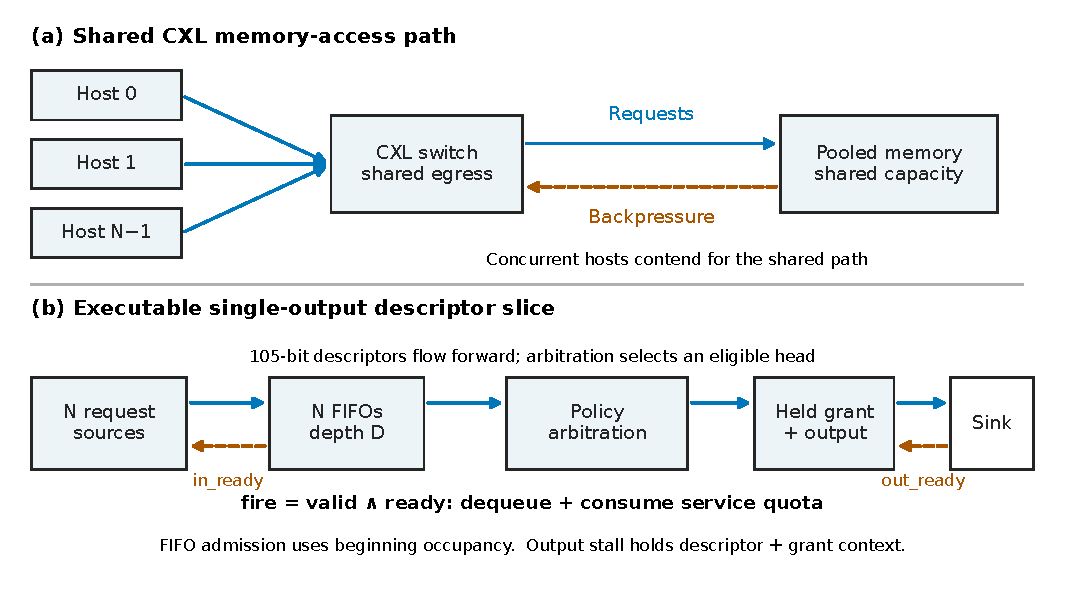
\includegraphics[width=\textwidth]{generated/figures/improvement/pooling-path.pdf}
\caption{Pooled-memory access path and evaluated single-output switch slice. CXL fabrics motivate the host--switch--memory boundary~\cite{cxl_intro,pond,fai}; the inset specifies this study's per-source depth-$D$ FIFO queues, 105-bit atomic descriptor format, and shared ready/valid output.}
\label{fig:pooling}
\end{figure*}

Figure~\ref{fig:pooling} isolates this contention boundary inside an executable single-output switch slice. Consider one \emph{Heavy} source issuing continuously alongside three \emph{Sparse} sources emitting occasional accesses. Under work-conserving saturation, aggregate output throughput barely changes between scheduling policies, yet waiting distributions diverge sharply. Giving Sparse arrivals earlier access slashes their tail latency while reshaping the spacing between consecutive Heavy grants. Because these stalls delay dependent processor loads on memory-access paths, arbitration choices must be weighed against both Heavy regularity and complete hardware area, timing, and power~\cite{cxl_intro,stfm,gupta}. System-level caching, DRAM bank timing, and application slowdown remain outside this switch-slice contract and require coupling with full-system simulators~\cite{cxl_interplay,contention_cache,hpc_pool,cxldmsim}.

Prior fairness-aware CXL scheduling (FAI-CXL) combines cacheline-weighted device interleaving with a windowed history classifier and transitional \emph{Buffer} state~\cite{fai}. When we reconstruct that classifier in executable RTL on a common N4/D16 switch boundary (Main), a telling anomaly emerges: Main cuts independent-arrival Sparse P99 delay nearly in half against FCFS (18.10 to 10.00 cycles), yet loses to simple quantum round-robin under bursty arrivals (21.05 vs.\ 17.70 cycles for RR10). Class-level alternation between High and Low turns forces three symmetric High sources to split half of all service opportunities while a single Low source claims the other half.

This paper asks how service history becomes a priority class, how priority classes map onto service opportunities, and what complete hardware cost implements those mechanisms cleanly. Our answer introduces Credit-Gated Oldest-First (CGOF), which decouples FAI's division-free classifier from per-source scheduling credits, alongside four diagnostic control studies covering allocation unit, absolute budget granularity, eligible-source ordering, and multi-window capacity and Buffer dynamics. We make three contributions:

\begin{enumerate}
\item \textbf{Common Executable Baseline and Burst-Reversal Diagnosis.} We construct a cycle-accurate RTL platform with fixed 105-bit descriptor storage, ready/valid stall holding, and independent Python reference models across FCFS, RR1/RR10, Main, \Alg{} (\code{Algorithm-2}), BLISS-inspired, and CGOF. We isolate why Main trails RR10 under bursts ($+3.35$ cycles) without blaming classifier delay.
\item \textbf{Causal Decomposition of Mechanism Axes (M1--M4).} Through targeted RTL and \code{MODEL\_ONLY} cohorts through November 7, 2026, we separate per-source credit ratios (M1), eligible ordering versus quota interaction (M2), absolute budget size versus spare-capacity absorption (M3), and Buffer hysteresis versus multi-window role switching (M4), plus a directed 512-cycle stall backlog drain verification.
\item \textbf{Complete Pre-Layout Hardware and Conditional Selection Map.} Using SAED32 RVT synthesis, equivalence checking, and thirty matched gate-level SAIF power captures (N4), we expose the area--power--regularity frontier across policies and formalize a conditional selection matrix with strict epistemic boundaries.
\end{enumerate}

Section~\ref{sec:fai} surveys related shared-resource schedulers and specifies FAI's dual Buffer semantics. Section~\ref{sec:rtl} defines the executable switch contract and CGOF. Section~\ref{sec:method} documents the experimental platform, updated evidence registry, and verification checks. Section~\ref{sec:results} steps through the causal mechanism diagnosis and hardware cost, and Section~\ref{sec:applicability} synthesizes selection rules, evidence limits, and open directions.

\section{Background, Related Work, and FAI Classifier}
\label{sec:fai}

\subsection{Shared-Resource Scheduling Landscape}
Packet switches and memory controllers establish two structural principles reused here. First, fixed-cost switch cell arbitration separates queueing mechanics from downstream fabric timing, as analyzed in crossbar schedulers~\cite{gupta}. Second, memory fairness policies judge cross-request interference relative to isolated execution (STFM)~\cite{stfm}, allocate service shares via fair queuing~\cite{fqmem}, rank threads by attained service (ATLAS)~\cite{atlas}, cluster bandwidth-sensitive from latency-sensitive threads (TCM)~\cite{tcm}, or temporarily blacklist streak-heavy requestors (BLISS)~\cite{bliss}. In weighted round-robin (WRR) arbitration for on-chip networks, Mandal et al.\ further distinguish allocated weight shares from short-term temporal ordering~\cite{wrr_mandal}. Our switch slice adapts explicit packet-cell arbitration, BLISS blacklisting, and WRR/IWRR baselines directly to equal-cost 105-bit descriptors without inferring DRAM row-buffer or cache-coherence behavior.

Within CXL pooling specifically, FAI-CXL joins a unified pool manager and cacheline interleaver with a windowed service classifier~\cite{fai}. Its scheduler monitors delivered service per host over fixed cycle windows rather than inspecting external queued demand. That feedback loop means classification reflects joint interactions among arrivals, FIFO admission backpressure, and earlier arbitration grants.

\subsection{Division-Free History Classification and Buffer Semantics}
For each source $h\in\{0,\dots,N-1\}$, let $B[h]$ count successful fires during the current $W$-cycle window, and let $S=\sum_{h=0}^{N-1} B[h]$. Comparing against the system-wide mean $S/N$ over all $N$ configured sources (inactive sources included) with threshold $\theta=0.3$, sources receiving below 30\% of average service generate \code{UP} evidence, those above average generate \code{DOWN} evidence, and ties or intermediate counts yield \code{KEEP}. Implemented without hardware dividers, the project classifier evaluates:
\begin{align}
\mathrm{UP}:&\quad 10NB[h]<3S,\nonumber\\
\mathrm{DOWN}:&\quad NB[h]>S,\label{eq:class-v3}\\
\mathrm{KEEP}:&\quad\text{otherwise}.\nonumber
\end{align}
This rule estimates recent delivered throughput rather than predicting future bursts or probing external producer queues.

\begin{figure*}[t]
\centering
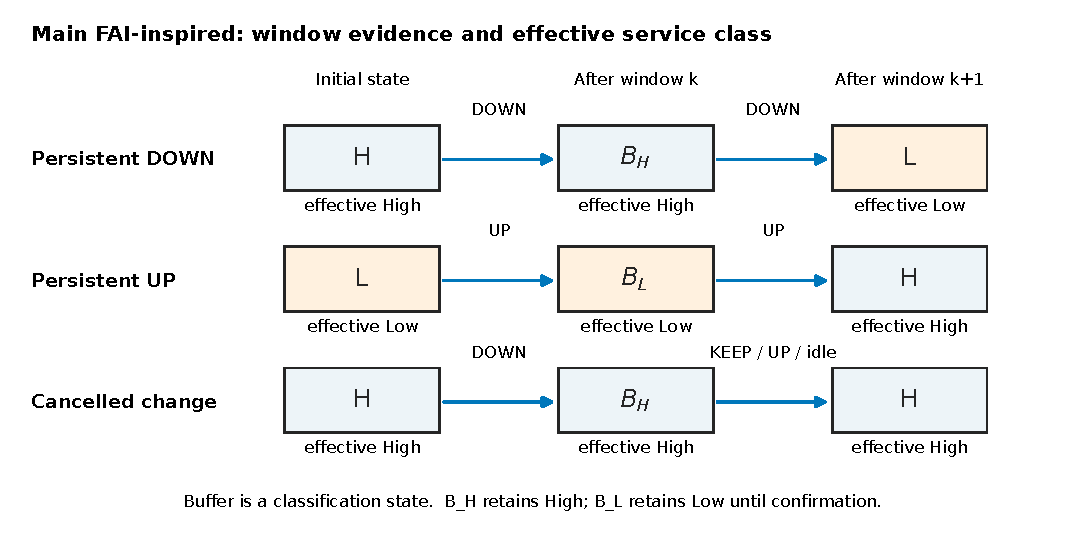
\includegraphics[width=\textwidth]{generated/figures/improvement/buffer-transition.pdf}
\caption{Classifier state semantics for Main's transitional Buffer ($H$, $B_H$, $L$, $B_L$)~\cite{artifact}. Two consecutive matching observations shift effective service class, whereas \code{KEEP}, opposite evidence, or an idle window ($S=0$) cancels a pending transition. Buffer holds classifier hysteresis state, distinct from request FIFOs.}
\label{fig:buffer}
\end{figure*}

Between High ($H$) and Low ($L$), FAI introduces transitional Buffer states ($B_H$ and $B_L$), yielding two distinct textual interpretations in the source paper~\cite{fai}. Section~IV-C of~\cite{fai} describes Buffer as hysteresis that preserves prior priority for one confirming window ($H\rightarrow B_H\rightarrow L$ requires two consecutive \code{DOWN} windows; a \code{DOWN} followed by \code{KEEP} returns $H\rightarrow B_H\rightarrow H$). Conversely, Algorithm~2 (lines 4--5, 13, 18 of~\cite{fai}) stores the new target priority into $P_{\rm last}$ upon Buffer entry and dispatches immediately using that target.

Because this distinction alters multi-window adaptation latency, we implement both cleanly: our primary reconstruction (Main) uses previous-effective-class hysteresis (Figure~\ref{fig:buffer}), treating $H$ and $B_H$ as effectively High and $L$ and $B_L$ as effectively Low, canceling pending moves on \code{KEEP} or idle windows. Our supplementary reconstruction, \Alg{} (\code{Algorithm-2} in archived artifacts), switches service class immediately upon Buffer entry while retaining Buffer state through \code{KEEP} and idle windows. Both preserve identical Eq.~\eqref{eq:class-v3} thresholds and 10/10 class turns. Section~\ref{sec:dynamic_conf} measures how these state rules trade noise rejection against settle time independently of queueing latency recovery.

\section{Executable Switch Contract and Policies}
\label{sec:rtl}

\subsection{Common Service and Stall-Hold Boundary}
Our hardware platform comprises $N\in\{4,8,16\}$ request sources sharing one output link ($D=16$ entries per source in primary builds; N4/D16 unless noted). Every FIFO entry stores the full 105-bit descriptor: 32-bit tag, 32-bit address, 1-bit opcode, 8-bit length, and 32-bit payload. Descriptor length fields remain intact across datapaths, while every fire transfers one atomic equal-cost request.

All compared policies execute over one shared ingress, queue, and stall-hold boundary (\code{switch\_top}):
\begin{itemize}
\item \textbf{Beginning-of-Cycle Eligibility:} Arbitration inspects queue occupancy at cycle start; a full FIFO rejects new pushes even if its head drains on the same edge, and newly admitted descriptors become eligible on the following cycle.
\item \textbf{Ready/Valid Output and Hold:} Successful transfer obeys:
\begin{equation}
\mathrm{fire}(t)=v_{\rm out}(t)\land r_{\rm out}(t).
\label{eq:fire-v3}
\end{equation}
Only $\mathrm{fire}(t)=1$ dequeues a head entry or consumes quota/credit. During $r_{\rm out}(t)=0$, a shared output-hold controller freezes the offered descriptor, source ID, and grant context; late arrivals cannot preempt a stalled offer, while non-full ingress queues keep admitting.
\end{itemize}

\subsection{Baselines and Class-Level Alternation (Main, \Alg{}, BLISS)}
\textbf{Timestamp-Free Round-Robin (RR1, RR10) and Global FCFS:} FCFS tracks 32-bit arrival timestamps per FIFO entry with modular wraparound comparison (valid for queue residence below $2^{31}$ cycles) and selects the oldest nonempty head globally. RR1 and RR10 eliminate timestamp arrays entirely, walking sources with a circular pointer and serving up to one or ten fires per visit while skipping empty queues.

\textbf{Windowed Class Schedulers (Main, \Alg{}):} Both maintain per-source 23-bit window counters $B[h]$, four-state classifications, class turn pointer and quota (10 High / 10 Low fires), 32-bit arrival timestamps, and stall-hold state. Within the active turn's effective class, the oldest eligible head wins (lower source ID breaks ties). When the active class has no ready heads, control immediately switches turns without inserting idle bubbles. All sources reset synchronously active-low to High, High turn first, over a production window of $W=5{,}000{,}000$ nonreset cycles (W5M, stalls included). On each closing cycle, hardware commits any $\mathrm{fire}(t)$ using the current grant context, updates $B[h]$ and $S$ with that final fire, computes Eq.~\eqref{eq:class-v3} via 32-bit unsigned products (preserving exact arithmetic up to $N=16$), and clears $B[h]$ and $S$; new classes take effect next cycle while stalled offers and active turn quotas survive across the boundary.

\textbf{Descriptor Blacklisting (BLISS-inspired):} Adapted from~\cite{bliss} without DRAM row-hit bias, BLISS-inspired favors non-blacklisted sources and chooses the oldest admitted head within that tier. Consecutive grants to the same source increment a streak counter; switching sources zeroes it. When an updated count exceeds four (meaning the sixth consecutive grant of a fresh streak), hardware blacklists the source and resets the streak. All blacklists clear every 10,000 cycles, with clear winning a simultaneous blacklist write.

\subsection{Per-Source Credit-Gated Oldest-First (CGOF) and Ordering Controls}
Why does Main lag RR10 under bursts? Because alternating 10-fire class turns allocates service at \emph{class granularity} (1/2 to all Low sources combined, 1/2 to all High sources combined), regardless of how many sources inhabit each class. When bursty Sparse sources interact across asymmetric class counts, class-turn boundaries serialize recovery unevenly.

CGOF breaks this coupling cleanly. It reuses Main's exact FIFO, timestamps, hold controller, and Eq.~\eqref{eq:class-v3} classifier, but discards class-level turns in favor of \emph{per-source local scheduling credits} (distinct from CXL link flow-control credits):
\begin{itemize}
\item \textbf{Eligibility and Refill:} A nonempty queue is eligible if its credit exceeds zero. Whenever no nonempty source holds positive credit, refill assigns every source fresh credit based on its current effective class: 1 each (High and Low) in CGOF (1:1), or 2 (High) and 1 (Low) in CGOF (2:1).
\item \textbf{Tie-Breaking, Commit, and Stalls:} Among eligible heads, the oldest timestamp wins (OF), with eligible round-robin (RR) isolated separately as an ordering control. Refill overwrites unused residual credits, never waits for empty sources, and triggers no double-refill on re-entry. Only $\mathrm{fire}(t)$ commits a refill snapshot and decrements the winning source's credit; stalled grants freeze their refill snapshot, and existing round credits persist across window transitions until the next refill.
\end{itemize}
Model controls additionally add fixed-weight round-robin (WRR) and interleaved WRR (IWRR) at weights $(2,1,1,1)$ to decouple target ratios from round spacing cleanly~\cite{wrr_mandal}.

\section{Experimental Platform and Verification}
\label{sec:method}

\subsection{Workloads, Metrics, and Cohort Registry}
Our primary N4 comparison runs 10M cycles across two W5M training windows with source~0 generating one Heavy request per active cycle. Arm~A (independent) generates Sparse requests on sources 1--3 at probability $1/128$ over 100,000 measurement cycles; Arm~B (bursty) issues 8-request bursts at seeded offsets per 1,024-cycle block across 100 blocks (800 requests per Sparse source), followed by a 1,024-cycle Heavy guard and full drain. Finite-Heavy studies parameterize \emph{under}, \emph{near}, and \emph{over} regimes via Heavy generation probability $p_{\rm Heavy}=0.25/0.80/1.00$, per-Sparse generation probability $p_{\rm Sparse}=0.02/0.02/0.05$ (aggregate nominal offered rate $\lambda=p_{\rm Heavy}+3p_{\rm Sparse}=0.31/0.86/1.15$), and sink readiness probability $0.90$.

For every request $i$, we measure generation cycle $g_i$, FIFO admission cycle $a_i$, and fire cycle $d_i$:
\begin{equation}
L_{GF,i} = d_i - g_i = L_{GA,i} + L_{AF,i}.
\label{eq:latency-v3}
\end{equation}
Here $L_{GA,i}$ captures external producer serialization and queue backpressure, while $L_{AF,i}$ captures local scheduler waiting (per-request exact, though marginal P99s need not sum). For each run, Sparse P99 pools completed Sparse requests generated before the active cutoff (including drain completions) and computes nearest-rank P99; reported cohort Sparse P99 averages those per-run P99 values across seeds. Note a critical finite-sample nuance: in short W256 runs, only $n=12\text{--}32$ Sparse requests complete per mixed run, so nearest-rank P99 equals that run's observed maximum, sharpening integer step effects compared to W5M.

Heavy interference is measured three ways: (i) uncensored FIFO-nonempty inter-service wall-cycle gap (consecutive fires have gap 1; startup, empty intervals, and right-censored segments excluded), tracking both gap P99 and each run's maximum gap; (ii) ready-opportunity gap under stalled sinks; and (iii) mixed-minus-isolated Heavy completion ratio and extra cycle delta $\Delta C = C_{\rm mixed} - C_{\rm isolated}$ (using paired exogenous arrivals and readiness traces~\cite{stfm}). For heterogeneous fixed-class controls we report weighted Jain's index (target $w_h/\sum_j w_j$) alongside Sparse-only and raw Jain's index.

All confirmation hypothesis tests use paired-seed 10,000-replicate bootstrap 95\% confidence intervals or pre-registered exact one-sided sign tests with Holm step-down ($\alpha=0.05$); descriptive and single-seed explorations report zero CIs. No repeated deterministic seed or in-run request inflates sample size. Table~\ref{tab:cohorts} separates every experimental cohort accepted through November 7, 2026 so confirmation, exploration, \code{MODEL\_ONLY} controls, and RTL anchors never conflate.

\begin{table*}[t]
\centering\footnotesize
\setlength{\tabcolsep}{4pt}
\begin{tabular}{@{}P{.27\textwidth}P{.22\textwidth}P{.47\textwidth}@{}}
\toprule
Cohort / Evidence Stream & Seed Set \& Scale & Scope, Boundary, and Inference Status \\
\midrule
Trained N4 RTL confirmation & 529--548 ($n=20$), D16/W5M & Paired A (independent) / B (bursty) after 2 windows across 6 baselines + CGOF (2:1) (\code{SCHEDULER\_RTL}). \\
Current-source CGOF (2:1) replay & 529--548 + 509--513 (30 runs) & Reproduces A/B ($n=20$) + Bernoulli 0.75 \& periodic 48/64 readiness ($n=5$, 60 endpoints, \code{SCHEDULER\_RTL}). \\
Single-factor \& 6201 RTL probes & 509--513 ($n=5$); 6201 (6 runs) & Descriptive fan-in (N4/8/16), RR quantum, Main High quota, depth (D8/16/32), burst stress; seed 6201 common-demand \& initial finite-Heavy 5M RTL (Sparse 3/4, max gap 9/10). \\
Allocation \& short model diagnosis & 6201--6220 ($n=20$) & 180 equal-demand + 100 fixed $L/H/H/H$ (20k cycles) + 300 finite-Heavy (20k, under/near/over), \code{MODEL\_ONLY}. \\
Near-load 5M finite-Heavy RTL & 529--548 ($n=20$, 80 runs) & 40 mixed/isolated pairs crossing 1 W5M boundary ($B_H/H/H/H$), CGOF (1:1) vs.\ (2:1) (\code{SCHEDULER\_RTL}). \\
Ordering RTL follow-ups (OF/RR) & 6501--6520 (W256, 160 runs); 6601--6605 (W5M, 40 runs) & W256 20-seed gate (7/20 $\le -1$, \code{NOT\_CONFIRMED}); W5M 5-seed descriptive exploration ($Q1/Q2\times\mathrm{OF}/\mathrm{RR}$). \\
Refill, lag \& Buffer model controls & 6201--6220 (80 pairs W5M); $5\times 4$ phases (W256 P0); 6101--6105 & Arrival-phase slack absorption (\code{MODEL\_ONLY}), deterministic refill trace (v2), 156 Buffer transition + 720 closed-loop runs. \\
4-window dynamic RTL probe & 7291 (1 seed, 20 runs) & 10 mixed/isolated W5M pairs (17.5M Heavy), role switch $[0,0,1,1]$, bursty stalls, D8/D16 (\code{SINGLE\_SEED}, CI null). \\
Dynamic role-switch confirmation + RTL anchors & 7401--7420 (600 \code{MODEL\_ONLY} jobs); 7301 (4 RTL), 7401 (2 RTL) & Pre-registered sign+Holm (P1--P3, $p=9.54\times 10^{-7}$, \code{MODEL\_ONLY}); Main exact-equality RTL anchors pass 4/4 (7301) \& 2/2 (7401). \\
Long-overload capacity absorption & 8101--8105 (60 \code{MODEL\_ONLY} jobs) & 30 mixed/isolated W5M 4-window pairs: under (4M Heavy, $p=0.25$) vs.\ over (17.5M, $p=1.0$, Sparse 0.05). \\
Directed 512-cycle stall drain & 7301 (Main, CGOF 1:1/2:1, 12 tests) & Cuts after 512-cycle \code{ready=0} stall (859 producer backlog + 64 FIFO); drains 923 requests to 0 (0 window closes). \\
Complete SAED32 hardware \& power & 9 primary + 6 CGOF configs; 509--511$\times$A/B (30 power runs) & Pre-layout DC/PT W-2024.09, TT 0.78V/25C, 25ns, formal equiv.; 18 primary + 12 matched CGOF zero-delay captures. \\
\bottomrule
\end{tabular}
\caption{Updated experimental evidence cohorts through November 7, 2026. Confirmation units (529--548, 6201--6220, 6501--6520, 7401--7420), descriptive explorations (509--513, 6601--6605, 8101--8105), single-seed probes/anchors (6201, 7291, 7301), and \code{MODEL\_ONLY} vs.\ \code{SCHEDULER\_RTL} tiers remain strictly separate.}
\label{tab:cohorts}
\end{table*}

\subsection{Pre-Layout Hardware Flow, Equivalence, and Drain Verification}
All synthesis and static timing analysis (STA) runs use Synopsys Design Compiler and PrimeTime W-2024.09 with SAED32 RVT (TT, 0.78\,V, $25^{\circ}$C, 25\,ns target clock) under identical external wire-load, timing uncertainty, I/O delay, and sink load assumptions. Reported cell area includes full descriptors, timestamps (when present), classifiers, quotas/credits, and shared stall-hold logic without FIFO blackboxing. Formal equivalence checks RTL-to-netlist correspondence cleanly (9,126 compare points pass for N4 CGOF (2:1)). Zero-delay ideal-clock SAIF power estimation evaluates seeds 509--511 across matched Arm~A (10,000,000 warmup plus 100,000 measured cycles) and Arm~B (10,101,024 warmup plus 102,400 measured cycles) traces. Constant-disabled \code{PTE-003} timing arcs (68 propagated arcs in N4 Main, \Alg{}, and CGOF netlists), FCFS/RR baseline static-pin power table-range qualifications, and wire-load optimistic fanout margins apply throughout and leave routing, SPEF, APR, and glitch unmeasured.

Cycle-accurate cocotb scoreboards and independent Python reference models verify transfer handshakes, FIFO admission, window closing updates, conservation ($\text{generated}=\text{accepted}=\text{fired}$), and stalled grant holds (463 CGOF matrix tests plus 17 model tests). Two dedicated hardware tests further validate cleanup and drain under queued backpressure:
\begin{enumerate}
\item First, the \code{depth8-bursty} anchor on seed 7301 halts active generation with requests still buffered and drains completely in 2 cycles ($\text{fired}=\text{accepted}=18{,}815{,}149$).
\item Second, a directed 512-cycle sink-stall test on seed 7301 (N4/D16, reset all-High, Main, CGOF (1:1), and CGOF (2:1), 12 tests passing 7/7 pipeline checks) holds downstream \code{ready=0} for 512 cycles (latched grant held 511 cycles), leaving 859 producer backlog entries ($[359,229,167,104]$) plus 64 FIFO entries (16 each). Upon restoring \code{ready=1}, all three policies drain in 923 cycles with per-source $\text{generated}=\text{accepted}=\text{fired}=[375,245,183,120]$ (923 total) and 0 outstanding. Because this directed fixture completes inside the first window (0 window closes), it validates datapath and drain safety rather than trained multi-window transitions.
\end{enumerate}

\section{Results and Causal Diagnosis}
\label{sec:results}

\subsection{Baseline Behavior and Why Main Reverses Under Bursts}
Figure~\ref{fig:confirmation-v3} establishes the central empirical puzzle across the twenty confirmation seeds (529--548, N4/D16, W5M). Under independent Arm~A arrivals, Main cuts Sparse G$\rightarrow$F P99 by 8.10 cycles relative to FCFS (18.10 to 10.00, paired 95\% CI $[-8.25, -8.00]$) and edges out RR10 (11.00, diff $-1.00$ $[-1.00, -1.00]$). Under bursty Arm~B arrivals, however, Main trails RR10 (21.05 vs.\ 17.70 cycles, diff $+3.35$ $[2.25, 4.45]$). \Alg{} closely tracks Main (10.00/21.35), proving immediate Buffer switching does not cure trained bursts, whereas BLISS-inspired achieves near-optimal Arm~A delay (1.15) at the price of FCFS-like burst tails (33.00 vs.\ 33.45) due to its 10,000-cycle clear cadence.

\begin{figure*}[t]
\centering
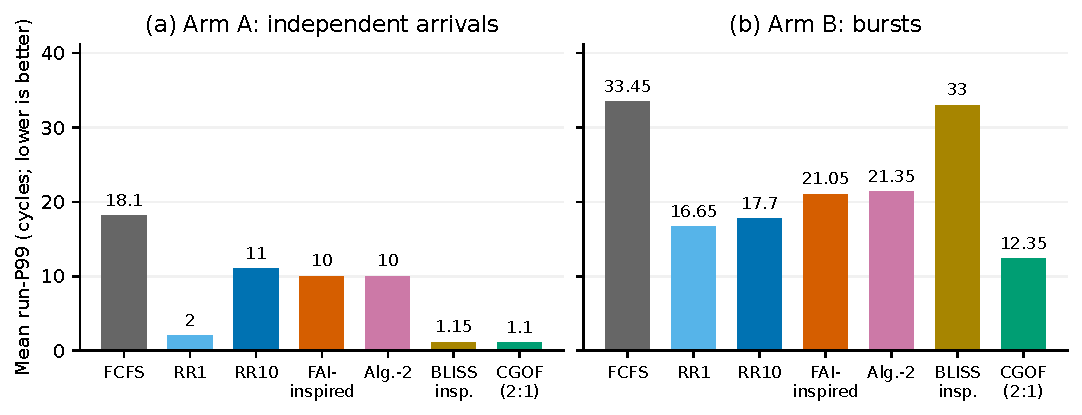
\includegraphics[width=0.88\textwidth]{generated/figures/confirmation.pdf}
\caption{Trained N4/D16 RTL confirmation (seeds 529--548, W5M): mean per-run Sparse generation-to-fire P99 (cycles). Main beats FCFS in both arms yet trails RR10 under Arm~B bursts ($+3.35$\,c). Decoupling per-source credits (CGOF (2:1)) drops P99 to 1.10/12.35 cycles ($-8.90/-8.70$ vs.\ Main, 20/20 seeds improve).}
\label{fig:confirmation-v3}
\end{figure*}

CGOF (2:1) resolves this burst reversal without changing link capacity, dropping Sparse P99 to 1.10 cycles (Arm~A, $-8.90$ $[-9.00, -8.75]$ vs.\ Main) and 12.35 cycles (Arm~B, $-8.70$ $[-9.50, -7.90]$), improving all 20/20 confirmation seeds in both arms. Moreover, in trained Arm~B (where Main already classifies Heavy as Low), CGOF (2:1) lowers the run-maximum Heavy wall gap from 11 to 7 cycles while Heavy wall-gap P99 shifts from 1 to 3 (fewer extreme stalls even as moderate 3-cycle gaps become slightly more frequent). Current-source RTL replays (Figure~\ref{fig:readiness-update}) reproduce the exact 1.10/12.35 means ($[1.00, 1.25]$ and $[11.80, 12.90]$) without altering paired provenance, and five-seed readiness sweeps show how stall temporal shape matters even at identical nominal 0.75 availability: Bernoulli 0.75 stalls yield 17.2/32.6 (Main) vs.\ 5.0/20.4 (CGOF (2:1)), whereas clustered periodic 48/64 stalls push tails to 26.0/34.0 vs.\ 17.0/27.0. Meanwhile, descriptive five-seed scaling to N8 and N16 leaves Main behind RR10 on Arm~B (27.60/34.80 vs.\ 21.00/24.40).

\begin{figure*}[t]
\centering
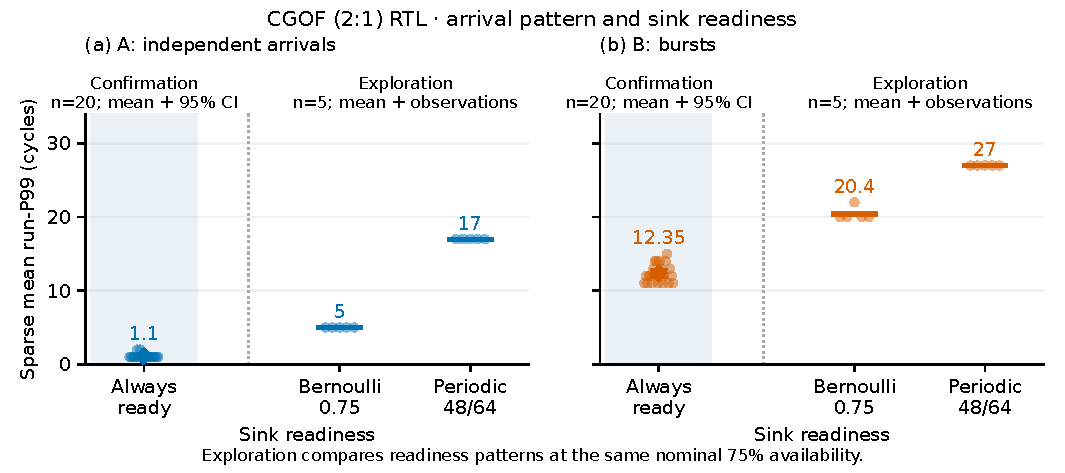
\includegraphics[width=0.86\textwidth]{generated/figures/update-20261029/readiness-confirmation.pdf}
\caption{Current-source CGOF (2:1) RTL replay across sink readiness models: 20 repeated always-ready confirmation seeds ($[1.00, 1.25]$ A, $[11.80, 12.90]$ B) plus 5-seed Bernoulli 0.75 (5.00/20.40) and periodic 48/64 (17.00/27.00) exploration.}
\label{fig:readiness-update}
\end{figure*}

\begin{figure*}[t]
\centering
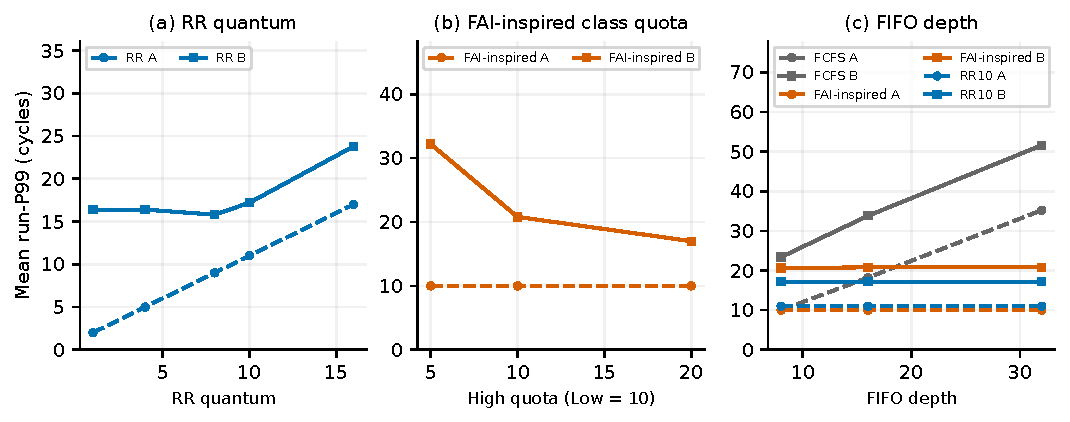
\includegraphics[width=0.86\textwidth]{generated/figures/sensitivity.pdf}
\caption{Descriptive single-factor RTL sensitivity (seeds 509--513, no CI) under trained A/B. Raising Main High quota from 5 to 10 to 20 shrinks Arm~B P99 ($32.2\rightarrow 20.8\rightarrow 17.0$ cycles); increasing depth D8 to D32 balloons FCFS Arm~A ($10.0\rightarrow 35.2$) while leaving Main and RR10 near 10--11.}
\label{fig:sensitivity-v3}
\end{figure*}

Why does Main lag RR10 on Arm~B bursts? Single-factor sensitivity (Figure~\ref{fig:sensitivity-v3}) points directly to quota structure: expanding Main's High quota from 5 to 10 to 20 slashes exploratory Arm~B P99 (32.2 to 20.8 to 17.0), whereas 32-request bursts stress Main to 88.8 (87.0 FCFS, 74.4 RR10). A production replay of seed 509 rules out classification latency as the primary culprit: after two training windows, sources already settle cleanly into Low/High/High/High, zero Sparse FIFO-full stalls occur, and yet seven High visits expire while High requests remain queued. Because fixed-visit offline reorderings over those turns also failed our improvement criterion, the root cause lies in \emph{how classes map to service quotas}, motivating our four mechanism controls below.

\subsection{M1--M2: Allocation Granularity (10/10 Class vs.\ Source Credits) and Ordering}
Figure~\ref{fig:allocation} (seeds 6201--6220, 20k saturated cycles initialized as Low/\allowbreak High/\allowbreak High/\allowbreak High before any window boundary) exposes M1 cleanly. Under continuous backlog, Main's 10/10 class turn forces equal 50/50 service between classes, yielding 49.9975\% to the single Heavy Low source and 16.6708/\allowbreak 16.6658/\allowbreak 16.6658\% ($\approx 1/6$) to each of the three symmetric High sources. CGOF (1:1) eliminates asymmetric class cardinality (25.0013/\allowbreak 25.0013/\allowbreak 25.0013/\allowbreak 24.9962\% over 20k cycles), while CGOF (2:1) shifts exact rational shares to $1/7$ (14.2857\%) for Low and $2/7$ (28.5714\%) for each High. Even at an all-High baseline control (20k cycles), WRR/IWRR $(2,1,1,1)$ achieves near-unity weighted Jain despite raw Jain near 0.893, proving that raw share inequality reflects assigned targets when backlog is uniform.

\begin{figure*}[t]
\centering
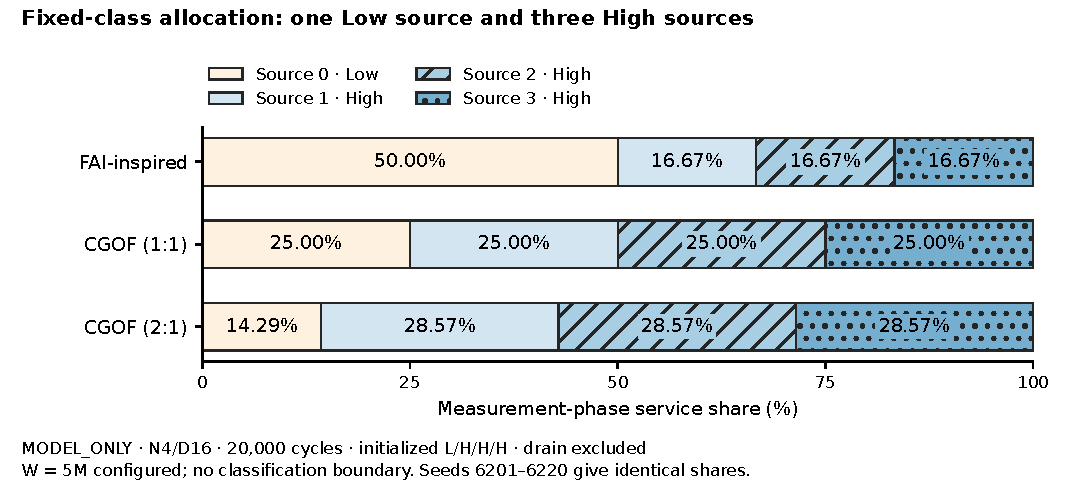
\includegraphics[width=0.88\textwidth]{generated/figures/improvement/allocation-shares.pdf}
\caption{Fixed-class saturation control (seeds 6201--6220, initial Low/\allowbreak High/\allowbreak High/\allowbreak High, \code{MODEL\_ONLY}, 20k cycles). Class-level 10/10 alternation (Main) grants about 50\% to one Low source and 16.7\% each to three High sources; CGOF (1:1) splits near 25\%, while CGOF (2:1) allocates 14.29\% Low and 28.57\% per High.}
\label{fig:allocation}
\end{figure*}

Class labels alone determine little without knowing the dynamic effective-class trajectory. In the 3-window common-demand RTL experiment (seed 6201, 256 external producer cap), bounded backpressure keeps all four queues equally fed ($B_H/\allowbreak B_H/\allowbreak B_H/\allowbreak H$ at boundary 1, $H/\allowbreak H/\allowbreak H/\allowbreak H$ thereafter; measurement fires 3,750,000 each except one 3,749,999, total 15,001,085), yielding symmetric P99 (1,086 cycles dominated by external producer queues) for both CGOF (1:1) and (2:1). Under intermittent arrivals, however, two credits versus one credit still diverge.

Does replacing oldest-first (OF) tie-breaking among credited sources with eligible round-robin (RR) provide an independent Sparse benefit (M2)? Figure~\ref{fig:ordering-v6} synthesizes both preregistered RTL campaigns crossing High:Low quotas Q1 (1:1) and Q2 (2:1) with ordering OF vs.\ RR under bursty 90\% readiness (N4/D16):
\begin{itemize}
\item \textbf{W256 Confirmation (6501--6520, 160 jobs):} With only $n=12\text{--}32$ Sparse completions per mixed run (so P99 equals run maximum), changing OF to RR leaves Q1 invariant ($d_1=0.00$ across all 20 seeds; Heavy max gap $\Delta=+0.00$, 0/20 diff) and cuts Q2 Sparse P99 by 1 cycle in only 7/20 seeds (mean $-0.35$, median 0; Heavy max gap $\Delta=-0.10$ in 2/20), missing the 15/20 gate (\code{NOT\_CONFIRMED}).
\item \textbf{W5M Exploration (6601--6605, 40 jobs, 5M Heavy):} Across all 5 seeds crossing one $H/\allowbreak H/\allowbreak H/\allowbreak H \rightarrow \allowbreak B_H/\allowbreak H/\allowbreak H/\allowbreak H$ boundary with zero censoring, Sparse P99 reads identically 11/11/12/11 cycles for Q1-OF, Q1-RR, Q2-OF, and Q2-RR ($d_1=0, d_2=-1, I=-1$). Yet RR increases Q1 maximum Heavy gap by $+1.6$ cycles ($+2,+2,+1,+2,+1$) while Q2 shifts $-0.2$ ($0,0,0,0,-1$), and extra completion delay $A=3,0,7,1,8$ cycles stays invariant (RR$-$OF $=0$ in 10/10). Ordering effects are therefore \emph{quota-dependent} and modest relative to per-source credit ratios.
\end{itemize}

\begin{figure}[t]
\centering
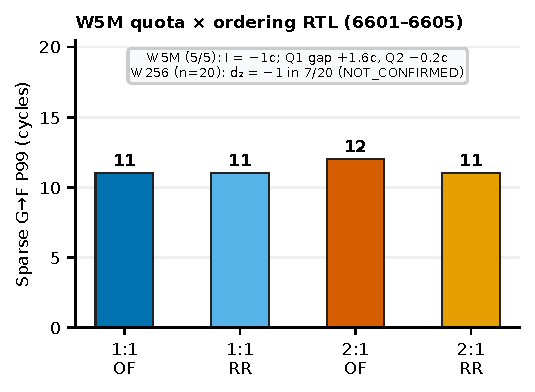
\includegraphics[width=\columnwidth]{generated/figures/v6/v6-ordering-panel.pdf}
\caption{W5M 5-seed quota$\times$ordering RTL exploration (seeds 6601--6605, $A=3,0,7,1,8$\,c invariant) against the W256 20-seed confirmation gate (6501--6520; \code{NOT\_CONFIRMED}). Ordering shifts Sparse P99 by at most 1 cycle and depends on credit quota (Q1 vs.\ Q2).}
\label{fig:ordering-v6}
\end{figure}

\subsection{M3: Absolute Budgets, Heavy Regularity, and Capacity Absorption}
Why do CGOF (1:1) and (2:1) differ when all sources hold effective High ($H/H/H/H$ or $B_H/H/H/H$)? Even though both prescribe equal target shares (1/4 each), absolute budgets set how many fires can accumulate before refill (1 vs.\ 2 per source). Deterministic trace \code{cxl-credit-refill-trace-v2} holds arrivals, stalls, and all-High classes identical while sweeping five Sparse arrival-phase offsets: three phases diverge at cycle 4 or 7 strictly through refill timing or eligibility shifts, proving absolute round size alters short-term dispatch ordering under intermittent load.

Figures~\ref{fig:tradeoff} and~\ref{fig:finite-confirmation} separate this budget effect under overload model contention (20k Heavy, all-High) versus near-load production RTL (5M Heavy, seeds 529--548):
\begin{itemize}
\item \textbf{Model Overload (6201--6220, \code{MODEL\_ONLY}):} CGOF (1:1) and (2:1) slash Sparse P99 from Main's 28.30 cycles down to 4.15 and 4.85 ($-23.45$ $[-23.80, -23.15]$ for 2:1; intermediate WRR and IWRR reach 10.00 and 8.70 Sparse P99 with 7.35 Heavy max gap and completion ratios 1.2003968/1.2004261), while mean maximum Heavy gap widens from 7.00 to 7.55 ($+0.55$) and 9.55 ($+2.55$ $[2.10, 3.00]$). Completion ratios stay tightly clustered (1.2002146 Main, 1.2004486 1:1, 1.2004373 2:1; $+0.0002227$ completion diff and $-0.0001544$ throughput-ratio diff for 2:1).
\item \textbf{Near-Load 5M RTL Confirmation (529--548, 40 pairs):} Against a nominal $\lambda=0.86$ offered rate vs.\ 0.90 sink readiness across one $B_H/\allowbreak H/\allowbreak H/\allowbreak H$ boundary, CGOF (1:1) beats (2:1) on both Sparse P99 (3 vs.\ 4 cycles, paired $+1.00$ $[1.00, 1.00]$) and mean maximum Heavy wall gap (9.45 vs.\ 10.85 cycles, $+1.40$ $[1.10, 1.75]$), while Heavy wall-gap P99 remains 3 cycles for both (showing percentiles can mask max-gap drift). Mixed Heavy completion exceeds isolated by only 3.05 $[1.45, 5.05]$ vs.\ 3.00 $[1.40, 5.00]$ cycles ($-0.05$ diff; ratio 1.000000488 vs.\ 1.000000480, Sparse-only Jain $\approx 0.999994$, Heavy 93.023\% of mixed fires). Finer 1-credit refills deliver superior temporal regularity below saturation.
\end{itemize}

\begin{figure*}[t]
\centering
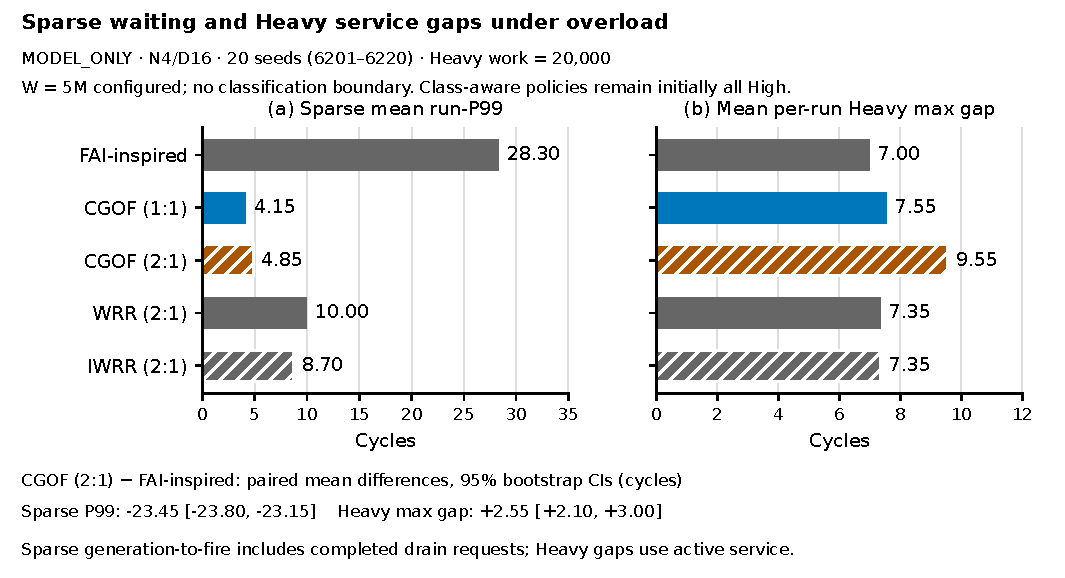
\includegraphics[width=0.87\textwidth]{generated/figures/improvement/heavy-sparse-tradeoff.pdf}
\caption{Short finite-Heavy model overload (seeds 6201--6220, 20k Heavy, all-High \code{MODEL\_ONLY}). CGOF (1:1) and (2:1) drop Sparse P99 from 28.30 to 4.15/4.85 cycles while raising max Heavy gap by $+0.55$ and $+2.55$ cycles and keeping completion ratios near 1.200.}
\label{fig:tradeoff}
\end{figure*}

\begin{figure*}[t]
\centering
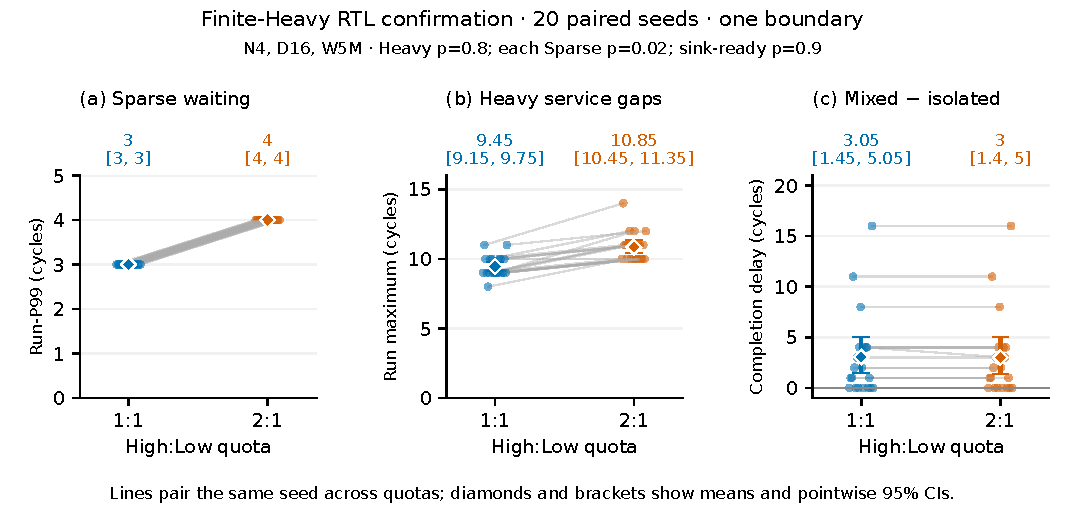
\includegraphics[width=0.87\textwidth]{generated/figures/update-20261029/finite-heavy-confirmation.pdf}
\caption{Twenty-seed near-load 5M RTL confirmation (seeds 529--548, 80 runs, 40 pairs, one boundary $B_H/\allowbreak H/\allowbreak H/\allowbreak H$). Smaller 1-credit rounds (1:1) outperform 2:1 on both Sparse P99 (3 vs.\ 4) and mean max Heavy wall gap (9.45 vs.\ 10.85), at nearly identical $+3.05/+3.00$-cycle extra Heavy completion.}
\label{fig:finite-confirmation}
\end{figure*}

Why does Sparse latency reduction cost almost zero Heavy completion near load yet extend completion under overload? Figure~\ref{fig:capacity-v6} resolves this conservation boundary (\code{MODEL\_ONLY}) without needing a duplicate table:
\begin{enumerate}
\item \textbf{Spare-Capacity Absorption (6201--6220 W5M \& P0 W256):} Under W5M under-load (6201--6220, 80 pairs), mixed-minus-isolated Heavy completion delay is 0.00 cycles $[0.0, 0.0]$ (ratio 1.000000; 20/20 inside the predeclared $\pm 20$-cycle equivalence margin). Under overload, delay climbs to $+834.25$ cycles $[820.4, 849.3]$ (ratio 1.037553, 0/20 inside margin). In the common-generation W256 P0 screen (5 seeds $\times 4$ phases), CGOF (1:1)/(2:1) incur mean max transient descriptor lag $\mathrm{lag}(k)=F_{\rm iso}(k)-F_{\rm mix}(k)$ of $1.25/1.25$ (under) and $5.00/4.95$ (near), recovering to 0.00 terminal $\Delta C$ (ratio 1.000000) in 20/20 runs, whereas overload leaves a $75.60/75.60$ descriptor lag and $+85.20$-cycle terminal delta (ratio 1.149956, 0/20 in margin despite 20/20 drain recovery).
\item \textbf{Long 4-Window Overload Conservation (8101--8105, Nov 7):} Across 60 \code{MODEL\_ONLY} jobs spanning four W5M windows (\code{heavy\_work=4M} under-load at $p_{\rm Heavy}=0.25, p_{\rm Sparse}=0.02$ vs.\ 17.5M over-load at $p_{\rm Heavy}=1.0, p_{\rm Sparse}=0.05$, sink readiness 0.90), under-load gives zero extra Heavy cycles (ratio 1.0, Sparse P99 4/3/3). Under long overload, CGOF (1:1) and (2:1) cut Sparse P99 from 27 (Main) to 4/4 and lower Heavy max wall gap from 18--19 to 11 and 13--14 cycles, while conserving aggregate Heavy completion time (ratio 1.200002 across all three; CGOF adds a mean of just $+0.4$ cycles ($[0,0,1,1,0]$) across a $\approx 3.889\text{M}$-cycle mixed-minus-isolated completion extension ($\Delta C$) on 17.5M Heavy work). Thus spare slots absorb Sparse service below saturation, whereas sustained overload obeys work conservation.
\end{enumerate}

\begin{figure*}[t]
\centering
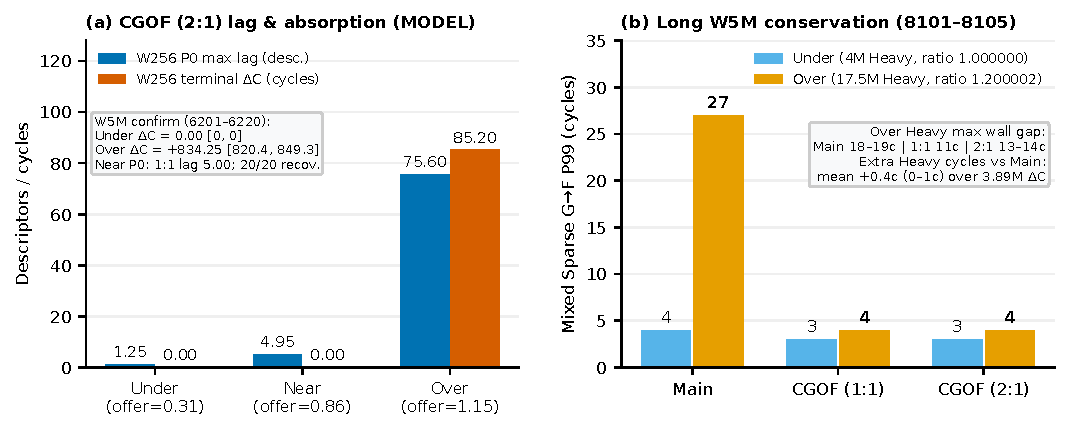
\includegraphics[width=0.91\textwidth]{generated/figures/v6/v6-capacity-slack-panel.pdf}
\caption{Capacity absorption and long-run conservation (\code{MODEL\_ONLY}): (a) CGOF (2:1) W256 P0 transient Heavy lag vs.\ terminal $\Delta C$ (CGOF (1:1) matches except 5.00 Near lag), annotated with W5M confirmation (6201--6220); (b) long 4-window W5M comparison (8101--8105), where CGOF cuts overloaded Sparse P99 $27\rightarrow 4/4$ (Main vs.\ 1:1/2:1) at conserved completion ratio 1.200002.}
\label{fig:capacity-v6}
\end{figure*}

\subsection{M4: Multi-Window Buffer Dynamics, Readiness Shape, and Role-Switch Confirmation}
\label{sec:dynamic_conf}

Extending beyond single-window controls introduces two multi-window effects: Buffer hysteresis timescale and workload role transitions. Because Main keeps previous effective class across one confirming window (10M cycles at W5M) while \Alg{} switches immediately (5M), isolated \code{MODEL\_ONLY} Buffer screens at W256 (78 transition-only replays per window across phases 0, 64, 255) confirm that Main rejects a one-window noise pulse (0 effective flips vs.\ 2 for Main-1W/\Alg{}) while taking 448--704 vs.\ 192--448 cycles to settle persistent role changes (varying with window evidence rather than fixed $2W$). Across 720 closed-loop W256 runs (6101--6105), CGOF (1:1) behaves identically across live, 1W, and frozen all-High classifiers in 120/120 scenario groups (confirming zero classifier leakage under equal credits), whereas CGOF (2:1) separates classifier settle delay from cohort waiting P99 without defining an explicit latency-recovery horizon.

\begin{figure*}[t]
\centering
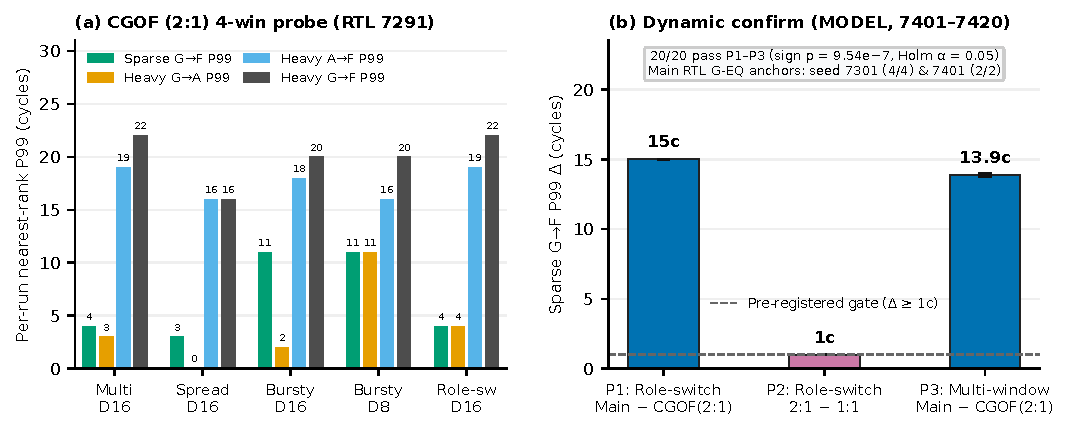
\includegraphics[width=0.94\textwidth]{generated/figures/v6/v6-dynamic-probe-panel.pdf}
\caption{Multi-window dynamic behavior: (a) exploratory single-seed 4-window W5M CGOF (2:1) RTL probe across all five test scenarios (seed 7291), contrasting baseline multi-window D16, stall clustering, D16 to D8 admission shifting, and role switches; (b) held-out 20-seed \code{MODEL\_ONLY} dynamic confirmation (7401--7420, 600 jobs) across contrasts P1--P3, anchored by Main exact-equality RTL runs on 7301 (4/4) and 7401 (2/2).}
\label{fig:dynamic-v6}
\end{figure*}

On a full 4-window W5M RTL trajectory (17.5M Heavy), the exploratory single-seed probe (seed 7291, 20 runs, 10 pairs, CI null, Figure~\ref{fig:dynamic-v6}a) spans five cases (starting from \code{Multi-window D16}: Sparse P99 3/4, Heavy $G\rightarrow A/A\rightarrow F/G\rightarrow F$ P99 4/19/22 and 3/19/22, wall/ready max gap 10/4 and 11/7):
\begin{enumerate}
\item Static runs evolve $H/\allowbreak H/\allowbreak H/\allowbreak H \rightarrow \allowbreak B_H/\allowbreak H/\allowbreak H/\allowbreak H \rightarrow \allowbreak L/\allowbreak H/\allowbreak H/\allowbreak H$, whereas rotating Heavy sources $[0,0,1,1]$ triggers three effective class transitions with full generation-role conservation.
\item At matched realized readiness (0.89999999 spread vs.\ 0.90000011 bursty), clustering stalls raises Sparse G$\rightarrow$F P99 and Heavy wall-gap P99 symmetrically from 3 to 11 cycles while Heavy ready-opportunity gap P99 holds at 2.
\item Halving FIFO depth from D16 to D8 under bursty stalls keeps Sparse P99 (11) and total Heavy G$\rightarrow$F P99 (20) fixed, shifting Heavy delay out of post-admission queueing ($A\rightarrow F$ P99: $18\rightarrow 16$) and into pre-admission producer backlog ($G\rightarrow A$ P99: $2\rightarrow 11$). Across all five seed-7291 pairs, CGOF (1:1) beats or ties CGOF (2:1) on Sparse P99 (3 vs.\ 4 on Multi-window/Role-switch; tied 3/11 on Readiness/D8), tightens max wall/ready gaps (9--14/4 vs.\ 11--17/7), and matches $\Delta C=+4$ to $+6$ cycles identically across 10/10 pairs.
\end{enumerate}

Finally, a held-out 20-seed dynamic confirmation (seeds 7401--7420, 600 \code{MODEL\_ONLY} jobs, N4/D16, 4 W5M windows, 17.5M Heavy, 24M cap, Bernoulli readiness) evaluates three pre-registered exact one-sided sign tests (1-cycle margin, Holm $\alpha=0.05$) directly on \textbf{mixed generation-time Sparse whole-run G$\rightarrow$F nearest-rank P99} (Figure~\ref{fig:dynamic-v6}b). All three pass in 20/20 seeds ($p=9.5\times 10^{-7}$): on role-switching (\code{src0} to \code{src1}), Main trails CGOF (2:1) by $+15$ cycles ($[15,15]$), and CGOF (2:1) trails CGOF (1:1) by $+1$ cycle ($[1,1]$); on multi-window fixed roles, Main trails CGOF (2:1) by $+13.9$ cycles ($[13, 14]$, descriptive CI $[13.75, 14.0]$). Although zero-width descriptive endpoints on P1/P2 reflect uniform nearest-rank P99 quantiles rather than general seed invariance, and 7401--7420 statistics remain \code{MODEL\_ONLY}, four W5M Main RTL replays on engineering seed 7301 (Sparse P99 19, null, 18, 19, including 2-cycle bursty-D8 drain) and two held-out Main RTL replays on 7401 (Sparse P99 19, null) match the Python model 4/4 and 2/2 on exact-equality gates (CGOF has no separate 7401 RTL replay).

\subsection{Pre-Layout Area, Timing, Equivalence, and Gate-Level Power}
Complete N4 cell-area decomposition reveals the physical price of timestamps and credit tracking. At N4, RR10 (79,047.172 library cell-area units) omits all ordering metadata and uses 27.65--28.20\% less area than Main (110,089.846) across N4--N16 (23.97\% less than FCFS's 103,970.058 at N4). Conversely, Main is 38.22--39.27\% larger than RR10. Table~\ref{tab:primary-area-v3} isolates disjoint N4 subsystems: descriptor storage fixes an equal 44,404.041-unit floor, timestamps add 13,532.660 units for FCFS/Main (8,192 bits alongside 26,880 descriptor bits by N16), and policy control grows from 263.039 (RR10) and 1,131.957 (FCFS) to 7,143.988 (Main).

\begin{table*}[t]
\centering\footnotesize
\setlength{\tabcolsep}{4pt}
\RevisionPrimaryAreaTable
\caption{Disjoint N4 cell-area decomposition (SAED32 TT / 25\,ns library units) from the primary leaf audit. Ordering timestamps (13,532.66) plus wider common selection account for Main and FCFS overhead over RR10.}
\label{tab:primary-area-v3}
\end{table*}

\begin{figure*}[t]
\centering
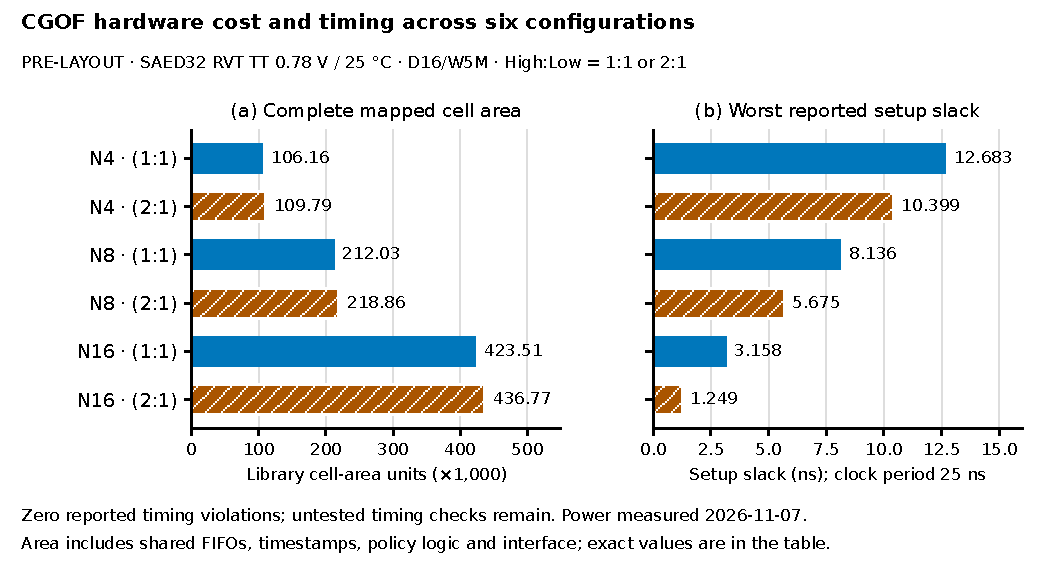
\includegraphics[width=0.80\textwidth]{generated/figures/improvement/cgof-hardware-v5.pdf}
\caption{Six complete pre-layout CGOF mappings (N4/N8/N16, D16/W5M, SAED32 RVT TT 0.78\,V / $25^{\circ}$C, 25\,ns). Area grows smoothly with source count ($106{,}163\rightarrow 423{,}513$ for 1:1; $109{,}795\rightarrow 436{,}771$ for 2:1); all six pass timing (lowest setup slack 1.249\,ns [exact 1.248813\,ns] at N16), with exact figures in Table~\ref{tab:cgof-hardware} and N4 power in Table~\ref{tab:power-summary}.}
\label{fig:cgof-hardware}
\par\vspace{2pt}
\centering\footnotesize
\setlength{\tabcolsep}{5pt}
\ImprovementCgofHardwareTable
\captionof{table}{Complete six-configuration CGOF cell area and STA (SAED32 RVT TT 0.78\,V / $25^{\circ}$C, 25\,ns, zero timing violations).}
\label{tab:cgof-hardware}
\end{figure*}

Figure~\ref{fig:cgof-hardware} and Table~\ref{tab:cgof-hardware} present all six complete CGOF synthesis/STA mappings (D16/W5M). All pass timing at 25\,ns: CGOF (1:1) spans 106,163.067 to 212,027.006 to 423,513.448 units (N4\slash N8\slash N16, setup slacks 12.683\slash 8.136\slash 3.158\,ns, hold slacks 0.035\slash 0.055\slash 0.078\,ns [exact 0.034898--0.078278\,ns]), while CGOF (2:1) spans 109,794.785 to 218,863.734 to 436,771.124 (setup 10.399\slash 5.675\slash 1.249\,ns, hold 0.039\slash 0.104\slash 0.084\,ns [exact 0.038578--0.103860\,ns]). CGOF (2:1) differs from Main at N4 by $-0.268019\%$ cell area (adding three flip-flops, 9,014 vs.\ 9,011, and passing all 9,126 formal compare points), while CGOF (1:1) saves 3.567\% area relative to Main; \Alg{} synthesizes within $-0.029\%$ of Main at N4 (110,058.332 units, 7,120.861 policy logic, 9,011 flip-flops, 10.547\,ns setup, 0.040\,ns hold). Because CGOF (1:1) weights Low and High identically, synthesis legitimately prunes classifier bits that cannot affect observable grants, leaving 138\slash 230\slash 414 matched unread accounting registers and 8\slash 16\slash 32 dead-state points disclosed cleanly in equivalence proofs. Pre-layout wire-load fanout caps can flatter setup slacks prior to physical clock-tree synthesis.

\begin{table*}[t]
\centering\footnotesize
\setlength{\tabcolsep}{2.5pt}
\begin{tabular}{@{}lccccP{.25\textwidth}@{}}
\toprule
Policy (N4/D16) & Internal A / B (mW) & Switching A / B (mW) & Leakage A / B (mW) & Total (mW) & Matched $\Delta$ vs.\ Main \\
\midrule
RR10 (3-seed mean) & 0.9995 / 0.9991 & 0.01345 / 0.01309 & 1.5467 / 1.5480 & 2.559--2.561 & $-26.1\%$ (2.560\,mW mean) \\
FCFS (3-seed mean) & 1.3060 / 1.3060 & 0.01781 / 0.01755 & 2.0320 / 2.0330 & 3.355--3.357 & $-3.2\%$ (3.356\,mW mean) \\
Main (3-seed mean) & 1.3317 / 1.3310 & 0.01920 / 0.01874 & 2.1160 / 2.1167 & 3.465--3.467 & 0.00\% (3.466\,mW ref.) \\
CGOF (1:1) (A/B range) & 1.328 / 1.328 & 0.01818--22 / 0.01793--94 & 2.069--70 / 2.069--71 & 3.415--3.417 & $-1.47\%$ to $-1.44\%$ ($+1.79\%$ FCFS, $+33.4\%$ RR10) \\
CGOF (2:1) (A/B range) & 1.331 / 1.331 & 0.01895--98 / 0.01858--59 & 2.112 / 2.112--14 & 3.461--3.463 & $-0.14\%$ to $-0.12\%$ ($+3.16\%$ FCFS, $+35.2\%$ RR10) \\
\bottomrule
\end{tabular}
\caption{Pre-layout gate-level zero-delay PrimeTime power (N4, SAED32 RVT TT 0.78\,V / $25^{\circ}$C, 25\,ns, seeds 509--511 across Arms A/B, 30 captures total: 18 baseline + 12 CGOF). For CGOF rows, Columns 2--4 list full Arm A / Arm B component ranges across seeds 509--511 (representative 509/A captures are 1.328/0.01818/2.069/3.416\,mW for 1:1 and 1.331/0.01895/2.112/3.462\,mW for 2:1); Column 6 summarizes paired within-trace totals.}
\label{tab:power-summary}
\end{table*}

Table~\ref{tab:power-summary} compiles the complete 30-capture N4 gate-level power comparison across seeds 509--511 and Arms A/B (completed November 7, 2026). Baseline 3-seed means sit at 2.560\,mW (RR10), 3.356\,mW (FCFS), and 3.466\,mW (Main). Across all six matched (seed, arm) traces, CGOF (1:1) consumes 3.415--3.417\,mW ($-1.47\%$ to $-1.44\%$ vs.\ Main [exact $-1.471\%$ to $-1.442\%$], $+1.787\text{--}1.788\%$ above FCFS, $+33.42\text{--}33.49\%$ above RR10; 509/A components 1.328/0.01818/2.069/3.416\,mW), consistent with dead-state pruning, while CGOF (2:1) closely tracks Main at 3.461--3.463\,mW ($-0.144\%$ to $-0.115\%$ vs.\ Main; 509/A components 1.331/0.01895/2.112/3.462\,mW).

\section{Discussion: Policy Selection, Scope Boundaries, and Future Work}
\label{sec:applicability}

\begin{table*}[t]
\centering\footnotesize
\setlength{\tabcolsep}{3.5pt}
\begin{tabular}{@{}P{.19\textwidth}P{.11\textwidth}P{.23\textwidth}P{.21\textwidth}P{.18\textwidth}@{}}
\toprule
Design Regime / Constraint & Policy & Primary Latency / Regularity & Hardware Cost (N4 vs.\ Main) & Active Evidence Tier \\
\midrule
No timestamps or dynamic classes needed & RR10 & Trained 11.00 / 17.70 (A/B); skips empty queues cleanly & $-28.20\%$ to $-27.65\%$ area (N4--N16); 2.56\,mW ($-26.1\%$ power) & Confirmed N4 RTL \& N4--N16 SAED32 \\
Single-boundary near load; fine round priority & CGOF (1:1) & 3-c Sparse P99; 9.45-c max Heavy gap; $+3.05$-c $\Delta C$ & $-3.567\%$ area; 3.415--3.417\,mW ($-1.47\%$ to $-1.44\%$); dead-state opt & Confirmed N4 near RTL; no 2:1 class differentiation \\
Asymmetric classes \& burst/dynamic protection & CGOF (2:1) & Trained 1.10 / 12.35 ($-89\%$ / $-41\%$); dynamic $-15 / -13.9$\,c (\code{MODEL}) & $-0.268\%$ area ($+3$ regs); 3.461--3.463\,mW ($-0.14\%$ to $-0.12\%$) & Confirmed N4 trained RTL; dynamic \code{MODEL\_ONLY} (Main RTL 7301/7401; CGOF RTL 7291) \\
Immediate 1-window flip preferred over filter & \Alg{} & 5M settle (W5M) vs.\ 10M for Main; trained 10.00 / 21.35; 2 noise flips at W256 (0 for Main) & $110{,}058.332$ units ($-0.029\%$); 9,011 regs; 10.55\,ns setup & Confirmed N4 trained RTL; Buffer \code{MODEL\_ONLY} \\
\bottomrule
\end{tabular}
\caption{Conditional policy selection matrix integrating queueing behavior, Heavy regularity, pre-layout hardware cost, and exact evidence boundaries.}
\label{tab:selection-matrix}
\end{table*}

No single policy dominates unconditionally across all metrics, workloads, and hardware budgets. Table~\ref{tab:selection-matrix} organizes our verified empirical results into a conditional selection guide:
\begin{itemize}
\item When dynamic history classes and timestamp ordering are unnecessary, RR10 delivers competitive burst latency (17.70 cycles) at the lowest N4--N16 cell area (27.65--28.20\% below Main, 23.97\% below FCFS) and power (2.559--2.561\,mW).
\item Under single-boundary near-load regimes where active classes collapse identically (1:1), CGOF (1:1) achieves the tightest measured RTL Sparse P99 (3 vs.\ 4 cycles) and lowest max Heavy gap (9.45 vs.\ 10.85 cycles) at $-3.567\%$ N4 area and $-1.47\%$ to $-1.44\%$ power vs.\ Main, though equal weights leave it unable to express 2:1 asymmetric differentiation when Low/High classes diverge.
\item Across trained asymmetric workloads and role-switch studies (\code{MODEL\_ONLY}), CGOF (2:1) corrects Main's Low-cardinality skew (14.29\slash 28.57\% fixed targets), cuts trained Sparse P99 by 41.3--89.0\% (12.35\slash 1.10 vs.\ 21.05\slash 10.00), and improves dynamic role-switch Sparse P99 by 15 cycles (\code{MODEL\_ONLY}) at nearly identical N4 area ($-0.268\%$) and power ($-0.14\%$ to $-0.12\%$) to Main. That gain trades $+0.55$ (1:1) and $+2.55$ (2:1) additional worst-case Heavy gap cycles in short 20k overload models (with $+0.0002227$ completion-ratio difference for 2:1), and trails CGOF (1:1) by 1 Sparse cycle in single-boundary near-load RTL and dynamic P2 role-switch models.
\end{itemize}

Four explicit scope boundaries bound every claim in this report:
\begin{enumerate}
\item \textbf{Tiered Inference Limits:} Queueing confirmation covers N4 W5M trained CGOF (2:1) (529--548), N4 single-boundary finite-Heavy CGOF (529--548), and the W256 ordering null (6501--6520, \code{NOT\_CONFIRMED}). Fixed-class shares, overload tradeoffs (6201--6220, 8101--8105), credit-refill divergence, Buffer transition screens, and 20-seed dynamic P1--P3 contrasts (7401--7420) are strictly \code{MODEL\_ONLY}, anchored only on Main (7301/7401) and single-seed 7291 dynamic RTL.
\item \textbf{Switch-Boundary Scope:} All latency metrics evaluate generation-to-fire scheduling ($G\rightarrow F$) for atomic equal-cost descriptors. End-to-end CXL.mem response time, DRAM row/bank timing, application bandwidth, and IPC slowdown lie outside this model~\cite{cxl_interplay,cxldmsim}.
\item \textbf{Hardware and Timing Scope:} Area, timing, and power reflect pre-layout, single-corner (SAED32 RVT TT 0.78V/25C, 25\,ns) synthesis and zero-delay SAIF activity; ideal clocks, wire-load models, disabled constant arcs (\code{PTE-003}), and absent SDF/APR/SPEF/glitch data prevent extrapolation to post-layout silicon energy or maximum frequency.
\item \textbf{Concrete Open Questions:} Closing remaining gaps requires (i) multi-seed multi-window CGOF RTL confirmation beyond single-seed 7291 and Main-only 7401 anchors, (ii) closed-loop variable-length and multi-channel DRAM/CXL simulator coupling, and (iii) post-place-and-route STA and physical clock-tree/power closure at N4--N16.
\end{enumerate}

\paragraph{AI use acknowledgment.}
Claude Code with RTL Agent Team and GPT-6.1 Sol assisted implementation and verification. GPT-6.1 Sol/high assisted prior manuscript drafting, evidence review, and figure production; Gemini 3.8 Flash/high reviewed language, and Antigravity assisted the v6 causal structural refactor and layout verification. Codex coordinated source verification, selective editorial integration, and PDF acceptance. Numerical claims derive strictly from the archived experiments and reports; the authors retain full responsibility for interpretation and final text.
